\chapter{Application Architecture}

\section{Data Model}



\subsection{DID, DID Document and DID-methods}
\begin{itemize}
\item A DID is the unique identifier of an agent.
\item DID's can resolve to a DID Document.
\item The DID-method decides the details on how to resolve the DID-document.
\item DID data model -> https://www.w3.org/TR/did-core/#data-model
\end{itemize}



\subsection{DIDKey method}

DIDKey is the only DID-method we are supporting. DID method key format -> https://w3c-ccg.github.io/did-method-key/#format



\subsection{ed25519-JWK}

The JWK DID-CLI is supporting, is a `ed25519/x25519` cryptographic public-private keypair, underpinning the DIDKey-method. The `jwk` is used for many things:
\begin{itemize}
\item Each unique `jwk` maps to a unique DID in the DIDKey-method.
\item By holding the `jwk`, the agent is able to assert control over it's DID in the DIDKey-method.
\item The `jwk` is used to encrypt DIDComm messages.
\item The `jwk` is used when generating the shared key in the Elliptic-Curve-Diffie-Helmann-key-exchange (ECDH-protocol).
\item The `jwk` is used to sign Verifiable Credentials and Verifiable Presentations.
\end{itemize}

\newpage

\begin{lstlisting}[
    caption={Example of an ed25519-jwk},
    label=lst:json,
    language=json]
{
	"kty":"OKP",
	"crv":"Ed25519",
	"x":"YRJAoEuAzcdc_7QdEM0NHQCd6hd-FdHkpdXl8T-RlVA",
	"d":"HOrwgKInYvPw_Wh6nN6kTNEd3wkkwYySMSuXzdr5Gec"
}
\end{lstlisting}

JWK format -> https://datatracker.ietf.org/doc/html/rfc7517#section-4.1



\subsection{DCEM - DIDComm Encrypted Message}

All messages read and written by the agent, are serialized as DIDComm Encrypted Messages, both in transit, and when at stored at rest inside the agent, as files.

DCEM spec -> https://identity.foundation/didcomm-messaging/spec/#didcomm-encrypted-message



\subsection{Verifiable Credentials}

All credentials issued by DID CLI are serialized as Verifiable Credentials.

    \begin{figure}[htbp]
      \centering
      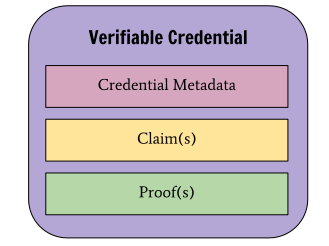
\includegraphics[width=.7\textwidth]{figures/credential.png}
      \caption[]{Illustration from https://www.w3.org/TR/vc-data-model/#credentials}
    \end{figure}



\newpage

\subsection{Verifiable Presentations}

All presentations presented by DID CLI are serialized as Verifiable Presentations.
    
    \begin{figure}[htbp]
      \centering
      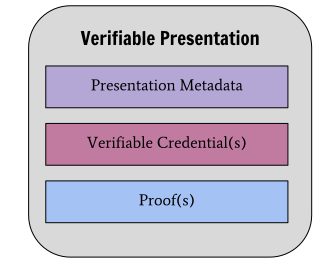
\includegraphics[width=.7\textwidth]{figures/presentation.png}
      \caption[]{Illustration from https://www.w3.org/TR/vc-data-model/#presentations}
    \end{figure}
    


\subsection{DIDName}
\begin{itemize}
    \item DIDName is a way of refering to a DID in a local DID-CLI command, because it is impossible to remember the full DID.
    \item DIDName is the only part of DID-CLI's data-model which is not part of an SSI-standard.
    \item Each DIDName is stored as a file `<DIDName>.did`, and the full DID as the content.
    \item Example: `self.did` or `jonas.did`.
\end{itemize}




\newpage


\section{File Storage}

\subsection{The .did/-directory}

All the agents files are contained within the `.did/`-directory, created when initializing the agent. The DID-CLI will use whatever `.did/`-directory is inside the current terminal working directory, just like GIT-CLI uses the `.git/`-directory.

\subsection{Portability}

The agent database, represented by the `.did/` directory, should be portable. A user should be able to move it to any other location on local machine, or to any other machine, and the agent should still work.


\subsection{One directory per agent}

\begin{lstlisting}[language=bash,caption={bash version}]

for i in bob lisa snorre jonas
do
	mkdir $i;
	cd $i;
	did init;
	cd ..;
done
\end{lstlisting}




\subsection{Communicating by sharing files}

\begin{lstlisting}[language=bash,caption={bash version}]
mkdir bob/ lisa/
cd bob/
did init
did did self > ../bob.did

cd ../lisa
did init
did did self > ../lisa.did

cd ../lisa
cat ../bob.did | did connect bob
cd ../bob
cat ../lisa.did | did connect lisa
\end{lstlisting}



\newpage


\section{High-level flow of scenario}

\subsection{Part 1 - The Government Issues credentials to it's citizens}


    \begin{figure}[htbp]
      \centering
      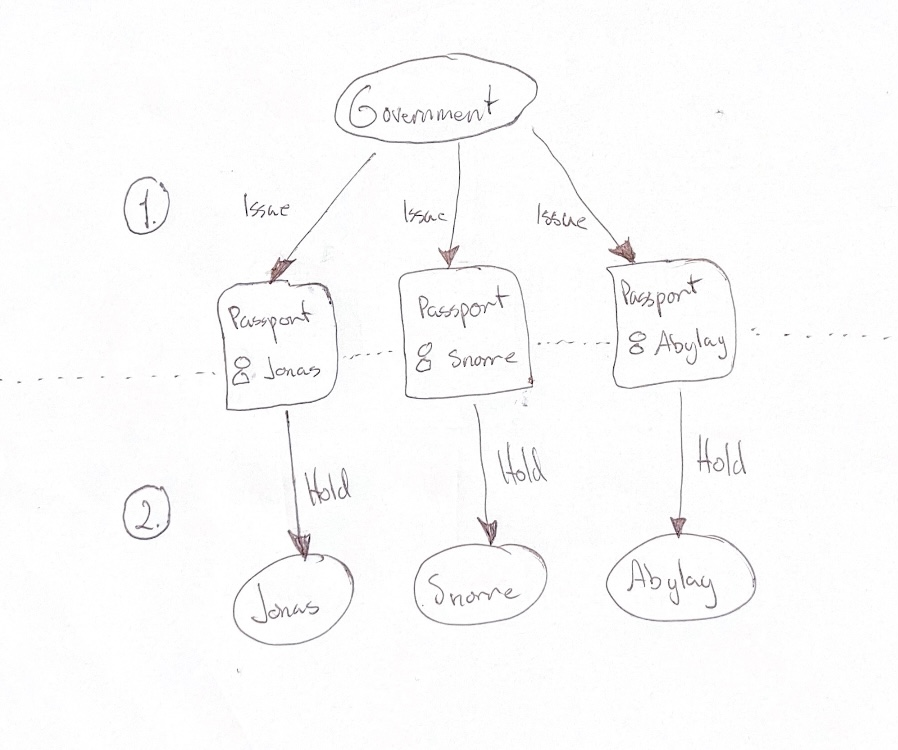
\includegraphics[width=.5\textwidth]{figures/scenario-1-2.png}
      \caption[]{Scenario Part 1 - Action 1 and 2}
    \end{figure}


\begin{description}
    \item[1. Issue:] The Government-agent issues 3 passport as Verifiable Credentials, to the 3 different citizen-agents - Jonas, Snorre and Abylay.
    \item[2. Hold:] The 3 citizen agents each hold the one passport issued to them.
\end{description}

    \begin{figure}[htbp]
      \centering
      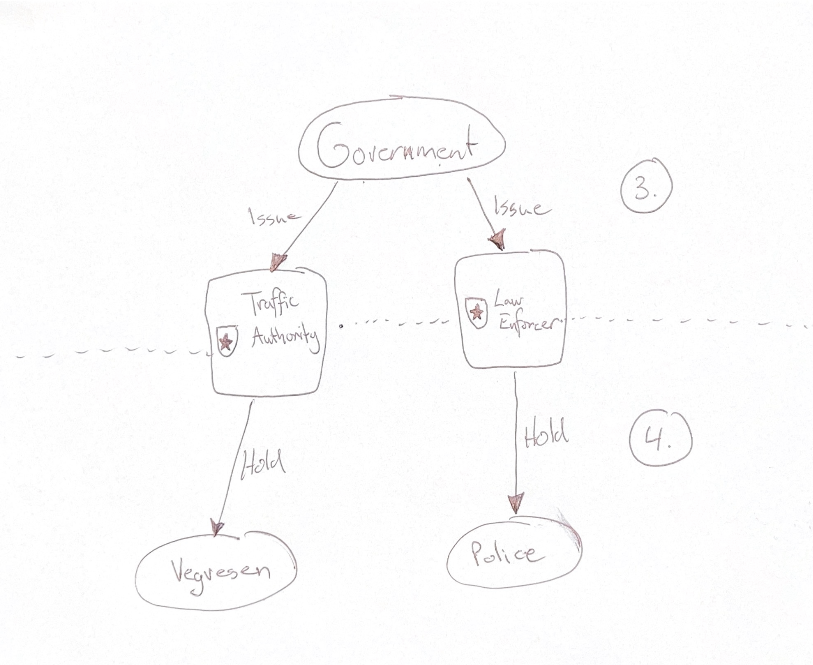
\includegraphics[width=.5\textwidth]{figures/scenario-3-4.png}
      \caption[]{Scenario Part 1 - Action 3 and 4}
    \end{figure}

\begin{description}
    \item[3. Issue:] The Govenment-agent issues a Traffic Authority and a Law Enforcer credential, to two different agents. This, in practice, creates the "Vegvesen" and the Police.
    \item[4. Hold:]The "Vegvesen"-agent and the Police-agent holds their respective credentials issued to them.
\end{description}


\newpage

\subsection{Part 2 - Jonas gets a Drivers License from Vegvesen}

    \begin{figure}[htbp]
      \centering
      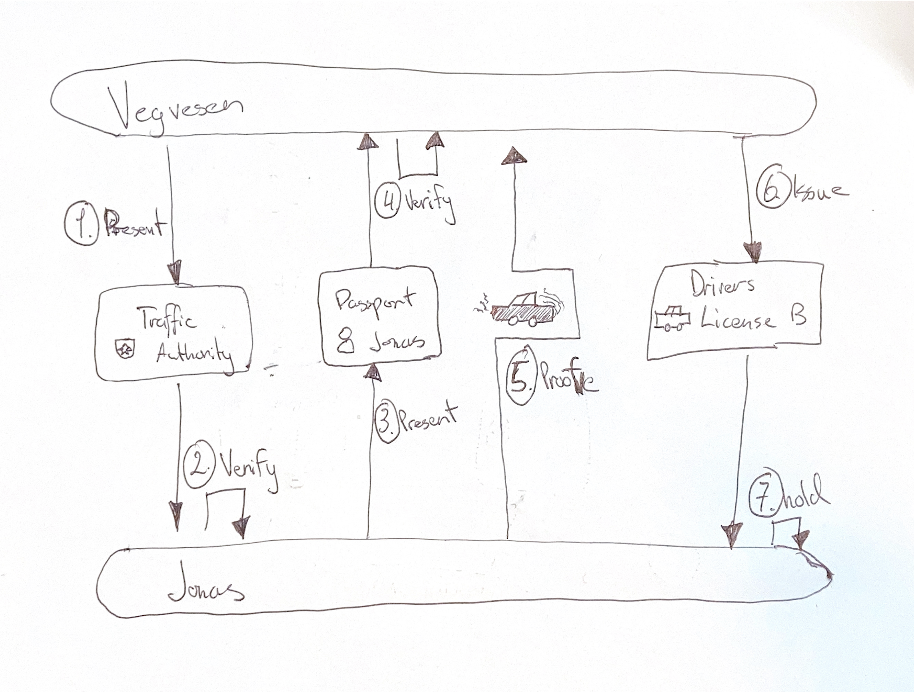
\includegraphics[width=1\textwidth]{figures/scenario-part2.png}
      \caption[]{Scenario Part 2}
    \end{figure}
    
\begin{description}
\item[1. Present:] - Vegvesen presents it's "Traffic Authority"-credential to Jonas,.
\item[2. Verify:] - Jonas verifies that the presentation has a valid signature, and makes sure that the "Traffic Authority"-credential was signed by the Government.
\item[3. Present:] - Jonas presents his "Passport"-credential to Vegvesen.
\item[4. Verify:] - Vegvesen verifies that the presentation is valid, and makes sure the passport credential was signed by the Government.
\item[5. Proove:] - Jonas somehow proves to Vegvesen that he know how to drive a car. This is out of scope of any of the SSI-protocols.
\item[6. Issue:] - Vegvesen issues a Drivers License as a Verifiable Credential to Jonas.
\item[7.  Hold:] - Jonas holds the Drivers License issued to him.
\end{description}


\newpage

\subsection{Part 3 - Jonas presents his Drivers License to Police}

    \begin{figure}[htbp]
      \centering
      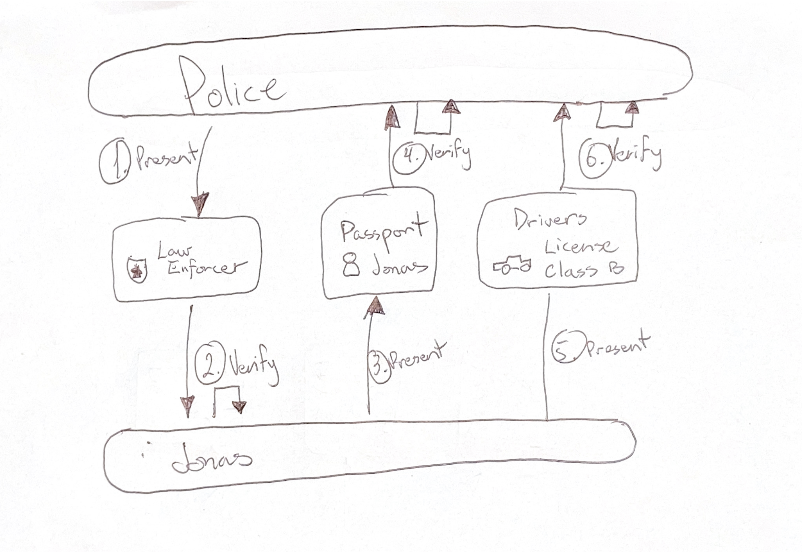
\includegraphics[width=1\textwidth]{figures/scenario-part3.png}
      \caption[]{Scenario Part 3}
    \end{figure}

\begin{description}
    
    \item[1. Present:] Police presents it's "Law Enforcer"-credential to Jonas.
    \item[2. Verify:] Jonas verifies that the presentation has a valid signature, and makes sure that the "Traffic Authority"-credential is issued by the Government.
    \item[3. Present:] Jonas presents it's Passport-credential to the Police.
    \item[4. Verify:] Police verifies that the presentation has a valid signature, and makes sure that the Passport-credential is issued by the Government.
    \item[5. Present:] Finally Jonas presents his Drivers License.
    \item[6. Verify:] Police verifies that the Drivers License is valid, and issued by the Government.
\end{description}
